\documentclass[12pt]{article}
\usepackage{graphicx}
\graphicspath{{Images/}}
\usepackage{textcomp} %for the copywrite symbol
%\linespread{1.6} %sets lines to 1.5 spacing.  1.6 would be double spaced
\usepackage[margin=1.0in]{geometry}
\usepackage[semicolon,round,sort&compress,sectionbib,numbers]{natbib}  
\usepackage{chapterbib}  
\usepackage{amsmath}
\usepackage{subcaption}
\usepackage{appendix} %for appendices
\usepackage{float}
\usepackage{listings}

\usepackage{hyperref} %make stuff clickable
\hypersetup{
	colorlinks,
	citecolor=black,
	filecolor=black,
	linkcolor=black,
	urlcolor=black
}


\usepackage{physics}  %for bras and kets!
\newcommand{\angstrom}{\mbox{\normalfont\AA }} %makes \angstrom do its thing!

\title{Lithium ELNES with WIEN2k}

\begin{document}
\maketitle

\tableofcontents

\section{Tools}	
Here's a list of software I use to run simulations.  I've put some installation instructions for linux as needed.  

\begin{itemize}
	\item Wien2k  - If you are reading this guide, you either already have it installed somewhere, or should figure out how to do that before buying a license.  
	
	\item  VESTA: \url{http://jp-minerals.org/vesta/en/download.html}.  Download the .rpm file, install it with your package manager, eg. ``sudo apt-get vesta...rpm"
	
	\item Critic2: \url{https://github.com/aoterodelaroza/critic2}.  Download the zip from GitHub, unzip where you want to install it eg $\sim$/Programs or something), install (using dnf/apt-get) autoconf, automake, and your favourite flavour of fortran.  Then run the 4 commands from the readme: ``autoreconf -i", ``./configure", ``make", and ``(sudo) make install".   You may or may not need the sudo for the last one. 
	
\end{itemize}
	
\section{Setup}	

We need a couple things to get started for ELNES simulations.  Foremost is a crystal structure.  You can either get this from the literature, XRD, or alternatively Materials Project: \url{https://materialsproject.org/}.  Download a cif (the primative cell typically) or enter the coordinates directly into the wien2k struct gen tool.  

Make a new Wien2k session: 
\begin{figure}[H]
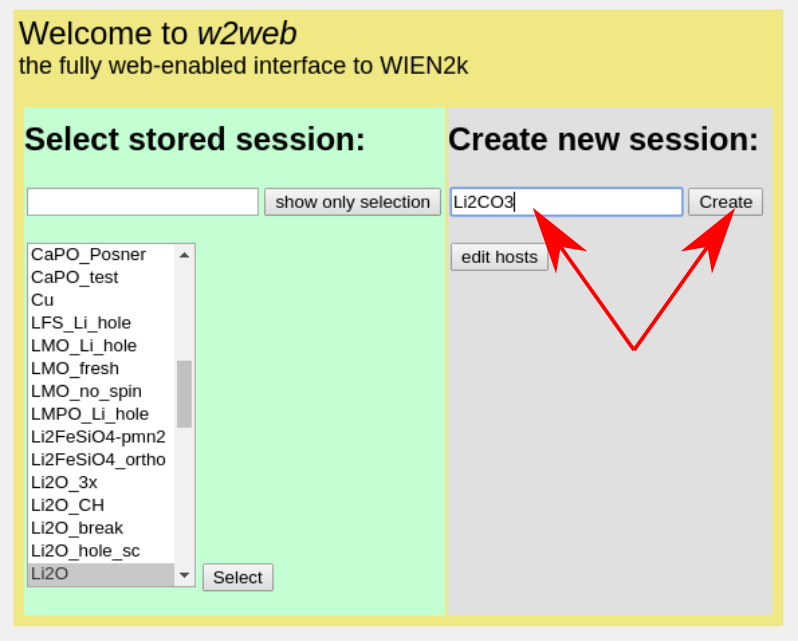
\includegraphics[scale=0.3]{./images/new_session.png}
\end{figure}

Create/change a working directory, and change the session information for parallel calculation.
	
	\begin{figure}[H]
		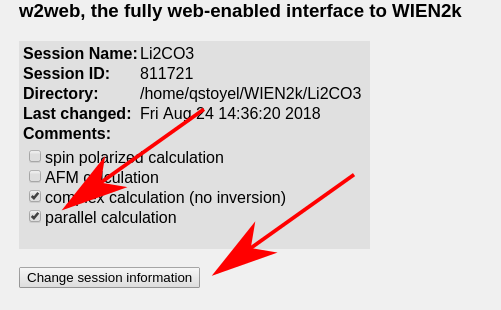
\includegraphics[scale=0.5]{./images/parallel.png}
	\end{figure}
	
You will also need to make a ``.machines" file which you can either steal from one of my directories, look in the user guide and make your own, cut and paste the one from below, or wait for w2web to automatically generate one at some point after it inevitably crashes on something.
Sample .machines file: 

\begin{lstlisting}
#=======================================
#This is a valid .machines file
#
granularity:1
1:localhost  #as many of these lines as you want cpu cores running
1:localhost  #ideally pick a multiple of kpoint number 
1:localhost  #so don't use 5 cores for 13 k points...
1:localhost
1:localhost
1:localhost

\end{lstlisting}

Next, go make a struct file, with struct gen, either by importing the cif, or entering the positions manually.  Use VESTA (drag n' drop the .struct file) to make sure that the structure is what you'd expect. 
In our Li2CO3 case this looks like: 

	\begin{figure}[H]
	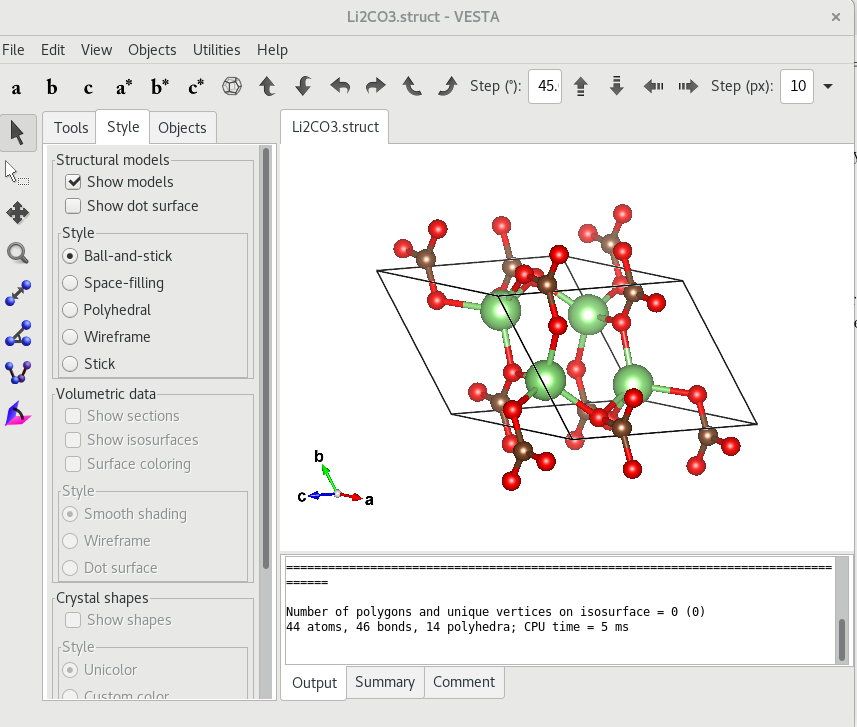
\includegraphics[scale=0.4]{./images/Li2CO3_struct.png}
\end{figure}


The next step is initialization.  This is best done via the command line as it give a little more flexibility and intuition than in w2web, and will need to be run multiple times.  Run \textbf{init\_lapw} and go through the following steps:

\begin{itemize}
	\item \textbf{setrmt}. Sets the muffin tin size on the atoms.  Reduce the sphere size by 0\% using either old or new scheme and accept, it doesn't matter much as these will be reset properly later.
	\item  \textbf{nn}.  Checks for overlapping muffin tins. Enter ``2.0", close the first file and use the new NN file if suggested, run \textbf{nn} with 2.0 again, look at how much ``wiggle room" you have on the spheres, by comparing the ``sums to" and the ``nn-dist" for every atom, see below:
	
	\begin{figure}[H]
		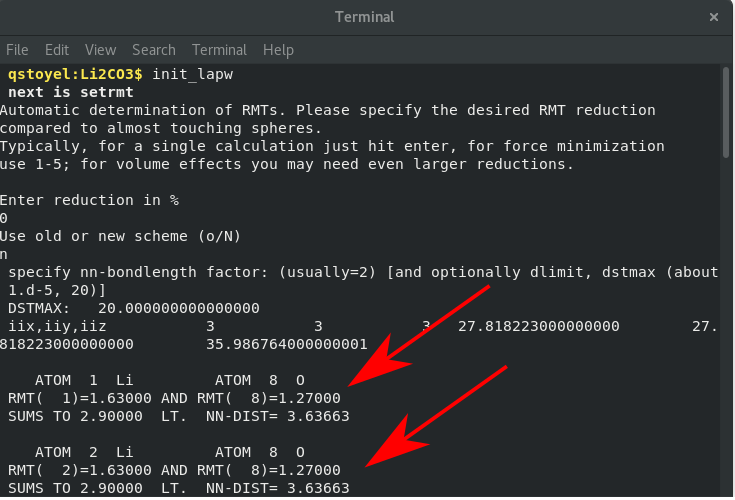
\includegraphics[scale=0.4]{./images/init_lapw2.png}
	\end{figure}
	
	\item \textbf{sgroup}. Verifies the space group.  Again, accept any changes the program makes, these steps are all about reducing the cell to the smallest unit cell. Again, the files can be largely  ignored at this point, with the exception of indication of a Bravais lattice change, in which case, accept the new struct file. If so, nn and sgroup will run again with ``nice" results.  
	\item  \textbf{symmery}. Generates all the symmetry operations. Run it and continue (enter ``c")
	\item  \textbf{lstart}. Set spin state, select which XC kernel, define cutoff between core and valence states.  Accept default spins (up, the no spin case), unless there is a transition metal involved. Select GGA PBE as the XC potential, again, unless there is reason to suspect otherwise. Picking the energy is the most important part of this first run init\_lapw: the aim is to get the Li 1s states to be treated as core states.  They typically have energies of $\sim$-3.7Ry, so try with -3.5 Ry to make sure they will be treated as core states and look in case.outputst (the file that pops up), for the following lines for the lithium atom and look at the 1S states:  
	
	\begin{lstlisting}
          E-up(Ry)      E-dn(Ry)   Occupancy   q/sphere  core-state
1S      -3.801947     -3.785288  1.00  1.00    0.9859  T
1S      -3.801947     -3.785288  1.00  1.00    0.9859  T
2S      -0.236699     -0.003313  1.00  0.00    0.0468  F
2S      -0.236699     -0.003313  1.00  0.00    0.0468  F
	\end{lstlisting}
	
	These indicate the core states (T/F), their energy levels (in this case $\sim$ -3.8eV) and how much the electrons in these states live in the muffin tins (0.9859).  As this is less than 1, it means a lot of 1S lithium electron is leaking out of the muffin tins, which is why there should now be all kinds of warnings popping up.  So go ahead and ``ctrl-c" out of init\_lapw.
	
\end{itemize}  

To fix the leakage problem, the Lithium muffin tins need to be bigger.   Ideally, they should be just big enough to hold all of the 1S electrons, without making them too different from the other muffin tins, as the larger this difference, the harder things get to calculate/converge.  In this case, try Li=1.8,  C=1.2, O=1.22 and try init\_lapw again, if that still didn't work (lstart still had leakage errors), keep going until it does, in this case RMT's of Li=2.0,  C=1.14, O=1.22.  These RMT values are too different ($\mathrm{RMT_{Li}} \approx 2\mathrm{RMT_C}$) and will cause errors  (ghostbands) further along.  The solution here is to try and minimize the leakage (and ignore the warnings) and acknowledge that it might be unavoidably causing artifacts. For this case I chose Li=1.8, C = 1.17, O=1.26. Alternatively, pick a nicer structure to analyze.  Once the spheres are set in the struct file, rerun \textbf{init\_lapw:}

\begin{itemize}
	\item \textbf{setrmt}: Setrmt will try to reset the muffin tins to the defaults, make sure to discard these (enter d)
	\item \textbf{nn} Make sure you don't get errors, and that everything is as tight as it can be, in this case the Oxygen-carbon spacing is the limiting factor.  
	\item \textbf{sgroup} Should run fine.
	\item  \textbf{symmery} Should run fine. 
	\item \textbf{lstart} Now that the lithium 1S states are well contained, core states can be selected based on containment instead of energy, meaning, the higher energy states (2S, P) of other elements can still be treated as valence.  Entering 0.99 should be sufficient here, but make sure to verify that the lithium states are still core states.
	\item \textbf{kgen} Set the RkMax value in case.in1\_st:		
	\begin{figure}[H]
		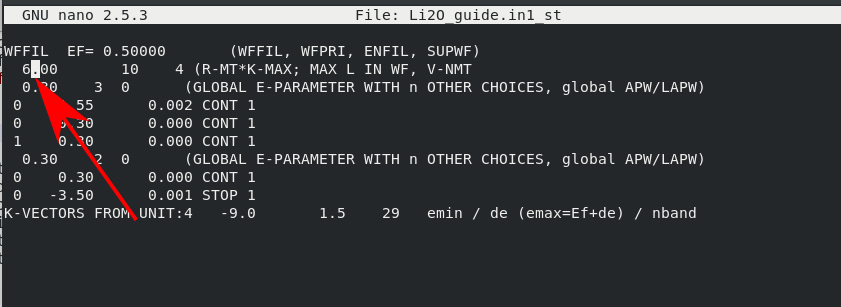
\includegraphics[scale=0.4]{./images/init_lapw3.png}
	\end{figure}
	and then pick a k\_point number.  Both of these values should initially be taken for fast convergence, in this case I chose RkMax=6.0, and 8 k points (Li2CO3 is an insulator, for metals 1000 k points is a good starting point).
	\item \textbf{Dstart}: make sure to pick non spin polarized, unless there is reason to believe otherwise (is there a transition metal in the sample?)
\end{itemize}

Assuming there were no warnings in the final run through init\_lapw, the case can begin to be converged.

\section{Convergence}
Ideally, every variable should be converged regarding the simulation.  Typically this is cell parameters, k points and Rkmax.  The first step is to just make sure the calculation converges, running it with a small RKmax and few kpoints and making sure it finishes without error.  

\subsection{Cell parameters:}
This process works best from W2Web, as described in the tutorials and using the muffin tins from \textbf{setrmt} reduced by a healthy percentage ($\sim$ 5-10\%) to avoid nn errors (you may need to rerun \textbf{init\_lapw}).    As  a number (5-11+) of calculations are run in this process, a low number of k points and RKMax values is ideal here. For Li2CO3, I used 16 kpoints and an RKmax of 6.   In the x ``optimize" tab, choose what you want to optimize, the first option (volume) works well, unless there are suspicions otherwise.  Enter a range of values of test volumes, see picture:

\begin{figure}[H]

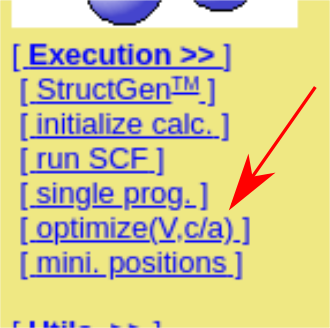
\includegraphics[scale=0.3]{./images/vol_opt_menu.png}
~
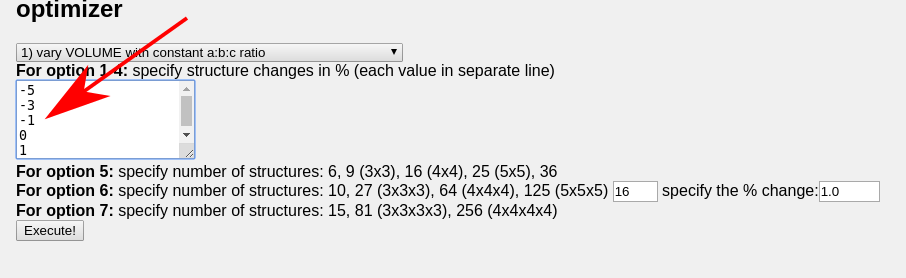
\includegraphics[scale=0.3]{./images/vol_opt.png}



\end{figure}


Also make sure to edit ``optimize.job" to enable parallization by moving the ``\#" to after the ``-p" in the run\_lapw line: 

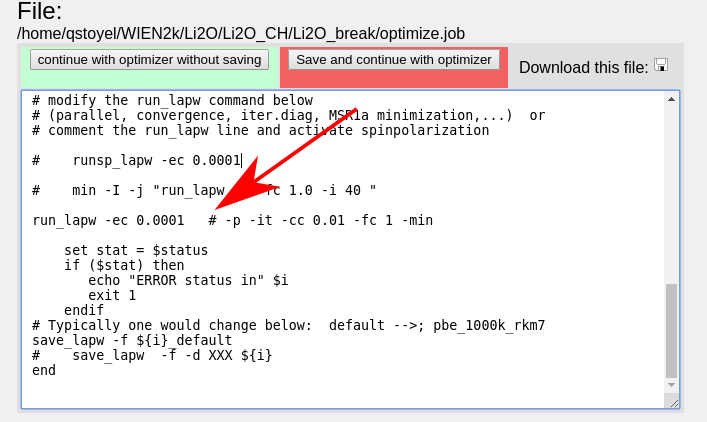
\includegraphics[scale=0.4]{./images/vol_opt2.png}

You can then ``run optimize.job" from w2web. This job is okay to run in the background, which means the browser can be closed without the job stopping.  When it is done, plot the ``Energy vs Volume," which should look something like this:\\
  
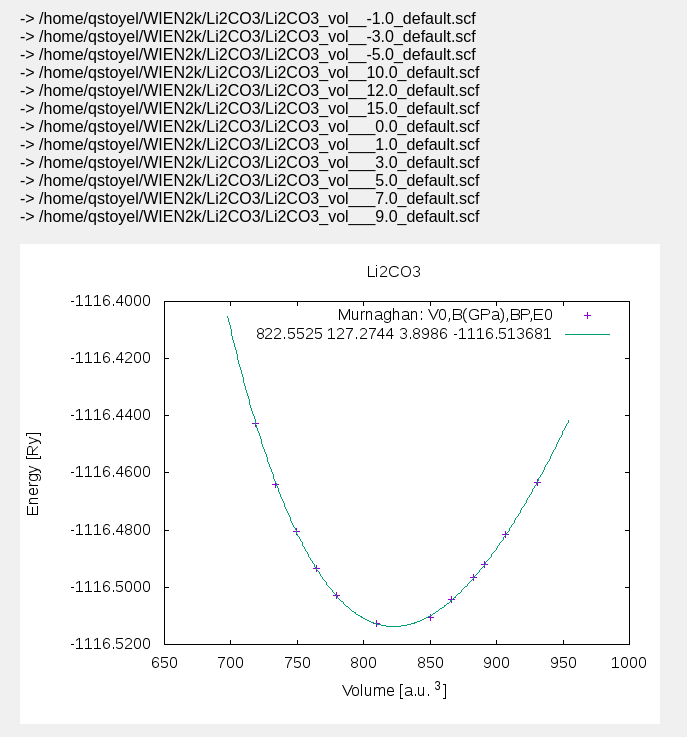
\includegraphics[scale=0.3]{./images/E_vs_V.png}

In the case of Li2CO3 and the cif from materials project, quite a range of volume options were needed to locate the minimum.  The graph indicates that a 3-4\% increase should correspond to the optimized structure.  To use this structure, search the case directory for all the struct files and rename the appropriate one to case.struct, for Li2CO3 this was ``Li2CO3\_vol\_\_\_3.0.struct $\to$ Li2CO3.struct". Alternatively, cut and paste the lattice parameters from this file into the w2web structgen tool.    Finally, rerun init\_lapw and readjust sphere sizes as necessary to account for the increase (or decrease) in cell size. 

\subsection{K point and RKMax convergence}

To converge these parameters, again start with very low values and then increase them, checking the total energy to determine when they are converged.  Generally k points are easier to converge, so start with them and then move on to RKMax. The procedure for converging both of these values is:

\begin{itemize}
	\item set/increase kpoints or RKMax, either by re-running ``x kgen" or editing case.in1 and case.in1\_st.
	
	\item Run the scf cycle using ``run\_lapw -p -NI", the NI flag means it will continue from where the previous calculation left off which saves time. I would still run your final choice from scratch though.
	
	\item Check the energy in case.scf.  To do this, find it in ``scf files" on w2web and use ctrl+f in your browser to search the file for ``:ene" , which should appear in a line that looks like: 
	
		\begin{lstlisting}
:ENE  : ********** TOTAL ENERGY IN Ry =        -1116.50733157
		\end{lstlisting}
	
	There will be one of these lines for each scf cycle, so find the last one in the document and note the energy. 
	
	
	\item loop through the first 3 steps until the energy no longer changes significantly when you increase the kpoints/RKMax.  A table is useful here to track these effects eg:
	
\end{itemize}

\begin{table}[H]
	\centering
\begin{tabular}{ccc}

			kpoints & RKMax & Energy \\
			\hline
			8 & 7.0 &  -1116.5073\\
			16 & 7.0 & -1116.4971\\
			32 & 7.0 & -1116.4975\\
			32 & 8.0 & -1116.5038\\
			32 & 9.0 & -1116.5045\\
			
			

\end{tabular}

\end{table}


\section{TELNES3}

Once the calculation is converged, ELNES can be calculated.  There is a good deal of useful information and a complete description of the input file in the wien2k userguide, which should solve most issues. Again, there is a large list of parameters that must be set for in order to obtain reasonable results. It is also worth converging Kpoints and RKMax against the spectra as well.\\
The majority of the important parameters need to be set in the \textbf{case.innes} file, which is easiest through w2web.  Choose the right atom (in this case Li1) for the edge, and the right atomic numbers:  

\begin{table}[H]
	\centering
	\begin{tabular}{ccc}
		
		Edge & n & l \\
		\hline
		K & 1 &0 \\
		L1 & 2 & 0 \\
		L23 & 2 &1\\
		M45 & 3 & 2\\
	\end{tabular}
	
\end{table}

Next, set the edge onset, edge values can be found at \url{http://www.kayelaby.npl.co.uk/atomic_and_nuclear_physics/4_2/4_2_1.html} as well as at a number of other locations.  Set the beam energy to it's correct value, same goes for the collection and convergence angles, although TELNES is relatively robust to these: eg 5mrad produces very similar results to 1 mrad.\\

Set the energy grid to a large range of values, eg -20-50eV so you can see all of the features that might appear.  The defaults for the remaining values should be fine.\\

In addition to the case.innes parameters, increase the number of kpoints, to at least double, or 10$\times$, so that there is less doubt about this being converged, use \textbf{x kgen} for this.  \\

Increase the upper energy limit in case.in1 from 1.5 to $\sim$ 2-3.5, see picture.  This value defines how many higher energy states are included in Ry (1 Ry $\approx$13.6 eV, 1.5Ry $\approx$ 20eV). Therefore, to obtain the correct ELNES for features more than 20eV from the onset,  this should be increased to match.  \\

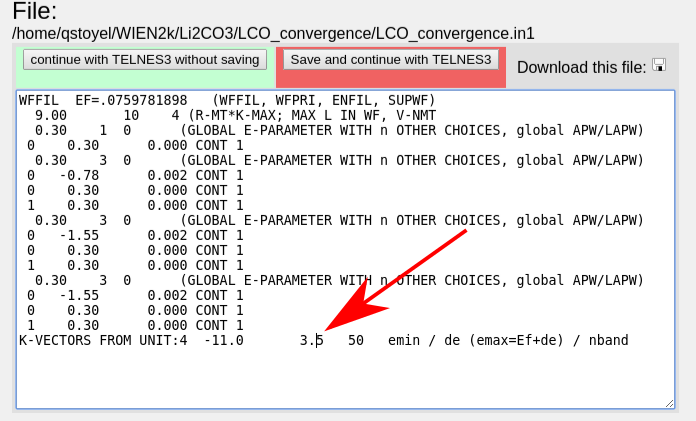
\includegraphics[scale=0.4]{./images/in1_edit.png}

\textbf{x lapw1 -p, x qtl -telnes -p}, and\textbf{ x telnes3} can then all be run in succession.  These are relatively slow commands, so to avoid waiting on them, run all three in sequence from the command line: \textbf{\$ x lapw1 -p \&\& x qtl -telnes -p \&\& x telnes3.}\\

Once telnes3 is finished, edit case.inb and play with the spectrometer broadening on the last line, before clicking ``x broadening" to generate the final spectra. To experiment with different broadening values, just repeat these steps.  Sometimes w2web gets stuck and stops re-broadening the spectra, in which case, just delete the case.broadspec file and run ``x broadening" again.   Plot the spectrum in a new tab (ctrl+click on ``plot") for easy comparison to new spectra without having to save it. Rerun all the TELNES steps, but with a higher/lower number of kpoints to confirm that that is not effecting the spectra. At this point you can also uncheck the ``calculate and write DOS" checkboxes in case.innes, which allow you to rerun telnes without needing to rerun\textbf{ lapw1} each time (unless you change the k points/case.in1 file).  If everything went well, the ELNES should look something like:   \\

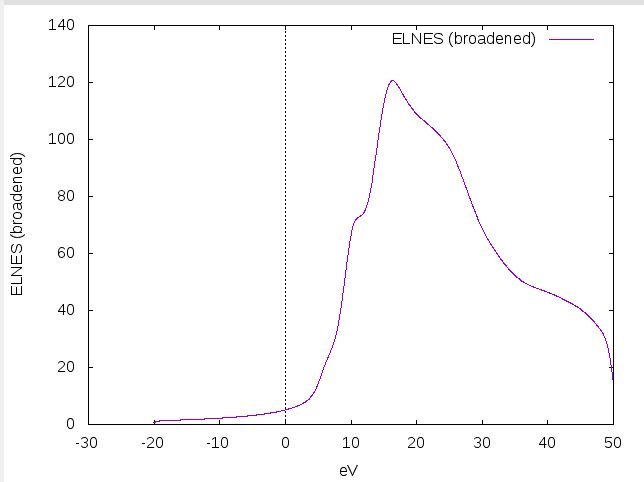
\includegraphics[scale=0.4]{./images/no_hole_elnes.png}

\subsection{Monopole effects}
Because the lithium 1S state is quite delocalized, it is susceptible to monopole effects.  These cause artifacts in the spectra resulting from non orthogonal states at the muffin tin boundary.  Fortunately, it is easy to check for them.  Return to the case.innes file and change the interaction order to 0. \\


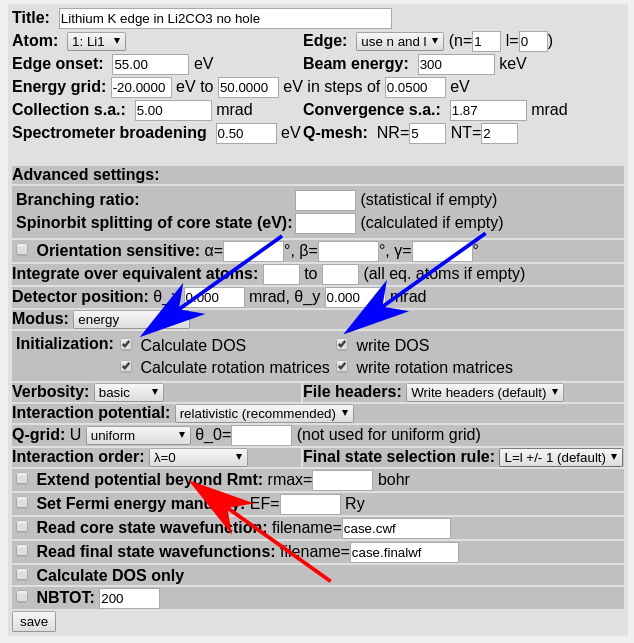
\includegraphics[scale=0.5]{./images/innes_monopole.png}

Telnes now only calculates the monopole component, look in case.outputelnes to confirm this.  Compare the monopole contribution to the full spectra, it should be much smaller ($\sim$100$\times$).  If it is not, set the interaction order to 1 to enforce dipole selection and use that for all future spectra.


\section{Core Hole}
To introduce a core hole, start an entirely new case, and copy only the struct file.  Because of the periodic boundary conditions, it is sometimes necessary to use a supercell to avoid core holes interacting with themselves in neighbouring cells. This depends largely on the size of the original unit cell, for a single atom case (metallic lithium) a 3$\times$3$\times$3 cell is required, for large calcium phosphates, no cell is needed. \\

Li2CO3 is a mid sized cell.  To verify that there is no interaction, the single cell case with a core hole will be compared to a 2$\times$1$\times$1 supercell.  If there is any significant variation in results a 2$\times$2$\times$2 supercell will be necessary.  \\

With all core holes, it is essential to remove the symmetry in the unit cell, so there is only a single hole per cell: 

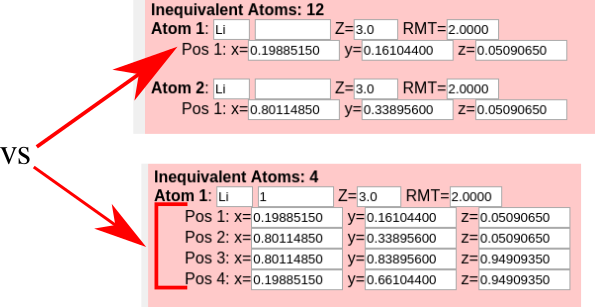
\includegraphics[scale=0.5]{./images/isolated_struct.png}

To achieve this, the cell must be reduced to a P1 space group.  This can be done in VESTA.  Import the struct file and set the space group to P1, under ``Edit $\to$  Edit Data $\to$ Unit Cell." Select space group No. 1, and apply. \\

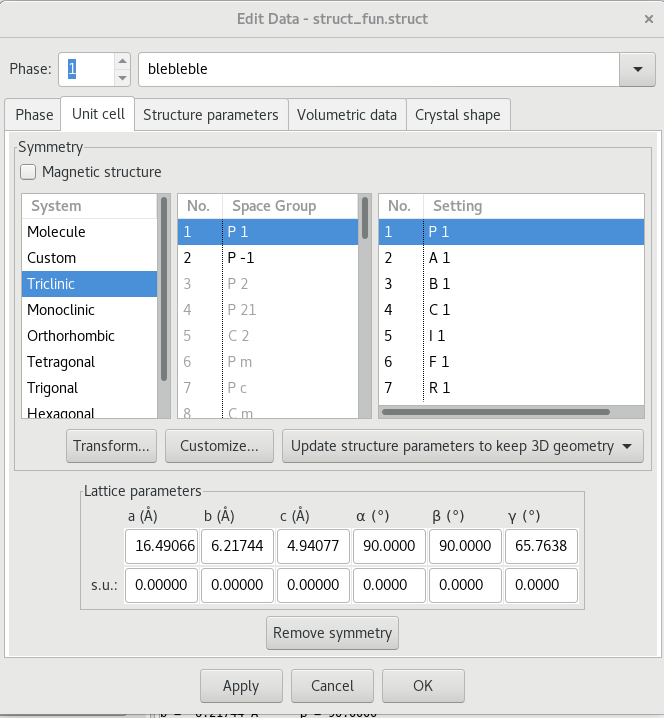
\includegraphics[scale=0.3]{./images/vesta_struct_edit.png}\\

 To save these changes select ``File $\to$ Export data" and save the structure as a .cif.  Because there are some bugs in the Wien2k-VESTA interface, the cif needs to be edited a bit manually as well.  Open the cif and delete the following line in the initial block of data: 

\begin{lstlisting}
_space_group_name_H-M_alt              'P 1'
\end{lstlisting}

and replace it with this line at the top of that block: 

\begin{lstlisting}
_symmetry_space_group_name_H-M   'P 1'
\end{lstlisting}

Running \textbf{Cif2struct name\_of\_cif.cif} should then be able to generate a valid struct file, which should be renamed as case.struct.  \\

In the new struct file, add a ``1" to the end of an atom (AND DELETE A SPACE).  The file should look like this: \\

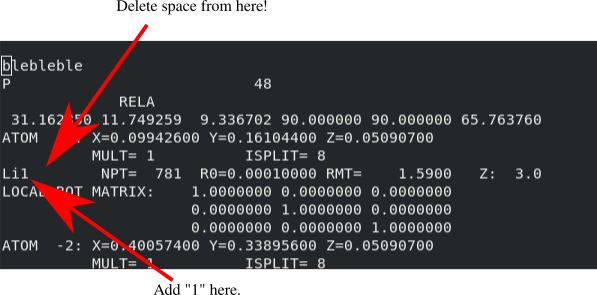
\includegraphics[scale=0.8]{./images/break_sym.png}
\\

Now run \textbf{init\_lapw} and accept all of the defaults proposed by \textbf{nn}, which may require cycling through \textbf{nn } a couple times.  \textbf{sgroup} should not have any suggestions here, if it does, something has gone wrong and it is trying to restore all of the symmetry.  At the end of \textbf{init\_lapw}, make sure to double check that the struct file is still what it should be.  


When the struct file is ready, initialize use the converged parameters (RMT, RKMax) from the single cell case.  After init\_lapw, insert a core hole into the cell by editing case.inc and case.inm: \\

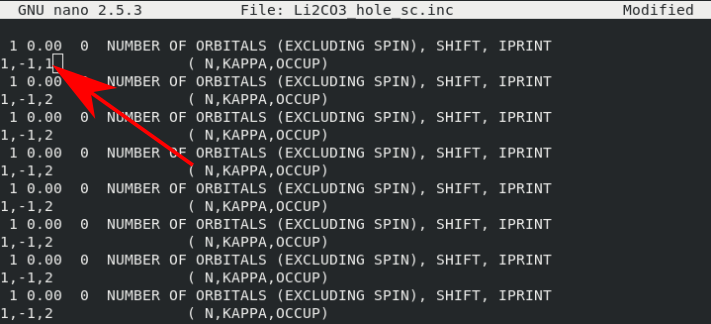
\includegraphics[scale=0.5]{./images/hole_inc.png}

In case.inc, a hole is inserted by changing the occupancy of an orbital.  Each set of lines corresponds to the core states of each atom defined in the struct file.  This is why it is important to be able to treat the lithium states as core states, otherwise it would not be possible to insert a hole.  This is also why it is important to break the symmetry in the unit cell as if not, this would insert holes into multiple atoms. In the case.inm file, the excited electrons need to be added to the background charge: \\

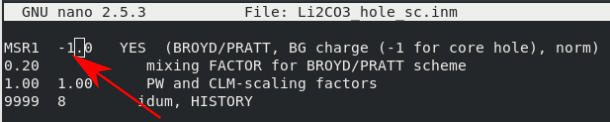
\includegraphics[scale=0.5]{./images/hole_inm.png}

The value is negative as this operation adds charge, not electron number.  Once the background charge is added, execute \textbf{run\_lapw -p} and calculate the ELNES.  If done correctly, your elnes should look something like this:  

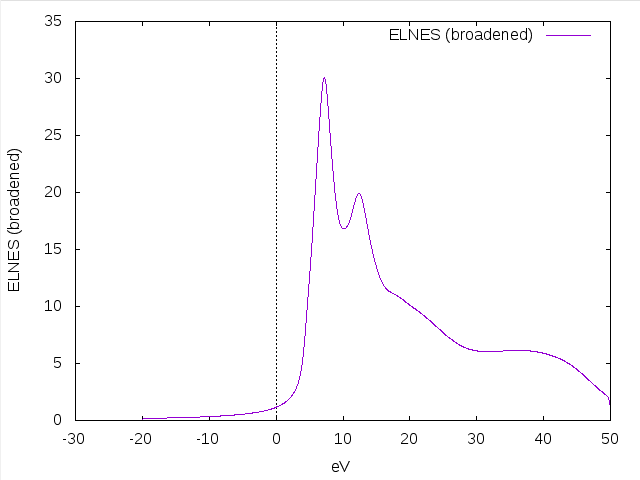
\includegraphics[scale=0.4]{./images/single_cell_hole_elnes.png}\\

To make a supercell, run \textbf{x supercell} in the directory and make a 2$\times$1$\times$1.  Then use the same procedure to keep the symmetry broken: import to vesta, select P1 spacegroup, save cif, edit spacegroup line in cif, cif2struct, relabel an atom with a number, and then run \textbf{init\_lapw}.  Reduce K points by a factor of 2 (the unit cell is now twice as big), and keep the RKMax from earlier.  Insert a hole in case.inc, case.inm and then \textbf{run\_lapw}.  



\section{Density Calculations}
Density calculations can be done using Critic2. Documentation for the code, while very complete, is just a giant txt file. The code takes three inputs: the case.struct file, the case.clmsum file, and an input parameters file ``more.cri".  A sample .cri file is below: 

\begin{lstlisting}
crystal ./Li2CO3.struct
load ./Li2CO3.clmsum ./Li2CO3.struct
auto
integrals gauleg 50 50 cp 1 verbose
sphereintegrals gauleg 50 50 cp 1 R0 1d-1 REND 2.0
\end{lstlisting}

The first line inputs the crystal structure, and then tells the code where to find the clmsum/struct files in the second line.  \\

The third line determines the location of all the critical points.  \\

The 4th line calculates the electron population inside the atomic basin surrounding critical point 1.  ``Gauleg" is a integration option, look in the critic documentation for more options.  The two 50's are sampling parameters, increase/decrease these for more/less accurate calculations.  \\

The 5th line calculates the electron population in spheres surrounding critical point 1. ``gualeg 50 50" mean the exact same as on the previous line, R0 is the starting radius, 1d-1 is the radius step size, REND is the final radius (in bohr).\\

The program is run using \textbf{\$ critic2 < more.cri > case.cro} in the command line in the case directory.  Te final file (case.cro) is just where the output is stored and can be called anything.  To determine which critical points are needed for the integrals, look at the complete cp list in the output file: \\

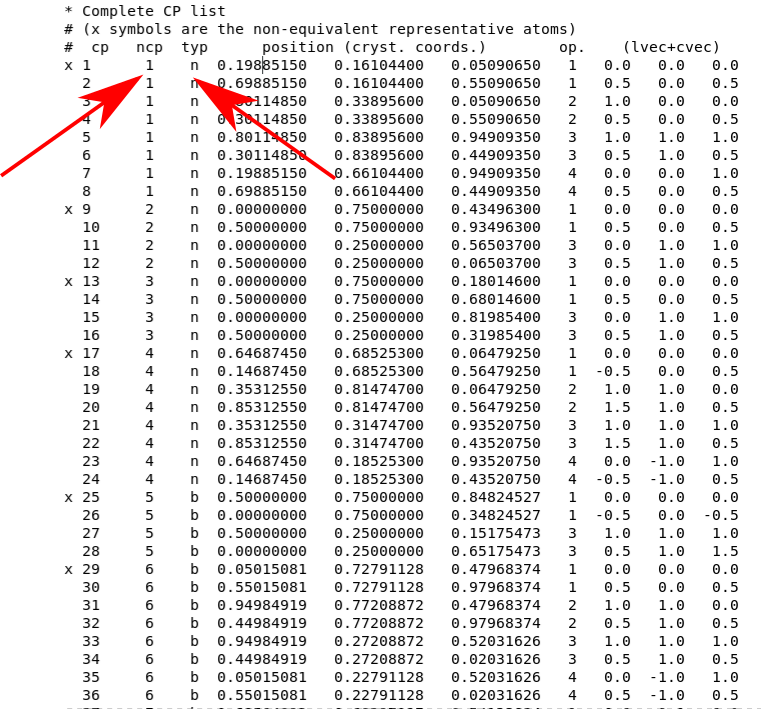
\includegraphics[scale=0.4]{./images/cro_cplist.png}\\

There are a number of similar lists which can be used to identify which atom is of interest.  The critical point should be a nuclear critical point (typ = n), and as a double check, the coordinates should match up to those in the struct file.  The name should also match, in this case, the ncp 1 corresponds to ``Li1."\\

The electron populations are located towards the bottom of the document.  The first case looks like this: \\

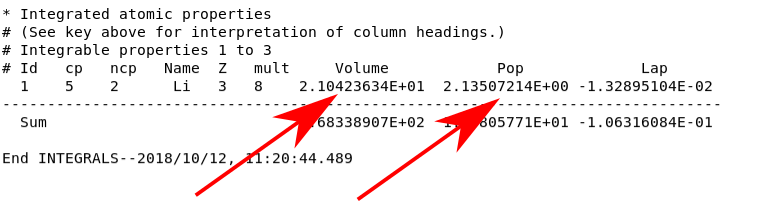
\includegraphics[scale=0.5]{./images/integrals.png}

The two values indicated by the arrows are the volume of the basin and how many electrons are inside. The second population is calculated directly below this in a table: \\

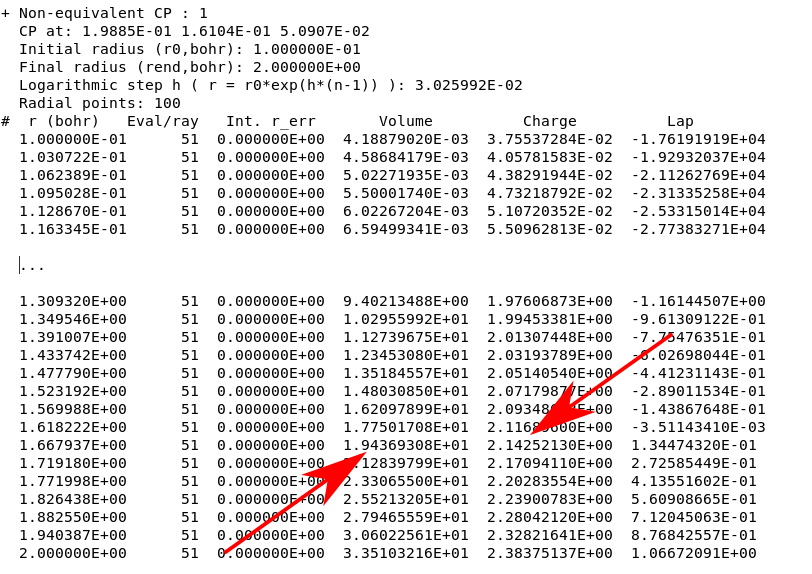
\includegraphics[scale=0.4]{./images/spheres.png}\\ 

By matching to the volume value, relatively comparable values should be attainable, in the no hole case.  The reason for performing two types of population calculation is due to the fact that the atomic basins can become ill defined when a core hole is inserted.  This is revealed when the volume of the basin is dramatically larger ($>$ 20\%) than the no hole case.  In these situations, a comparison of the sphere integrals at the same volume (set by the basin volume in the no hole case) is more appropriate.  \\

Once density calculations are performed for both hole and no-hole cases, core hole screening can be calculated by comparing the values.  For example if the no-hole population is: 2.17, and the core hole population is 1.5, the hole would be screened by:  (1.5 + 1) - 2.17 =  0.33 electrons. The +1 is to account for the excited electron.  To implement this effect, a third, final supercell calculation is required,  with a reduced hole inserted.  case.inc would need an occupancy of 1.33 and case.inm would need a background charge of -0.67. \\

\section{Common Errors/Issues Encountered in Wien2k}

\subsection{Setting RMT/RKMax}
The RKMax value is a little obscure and takes some getting used to.   It is defined as the Muffin Tin Radii $\times$ Maximum K point vector.   The maximum k point corresponds to the highest frequency plane wave used in the calculation. RKMax defines a cutoff for sampling  k space, based on the size of each atom.  A visualization of this effect is depicted below:

\begin{figure}[H]
	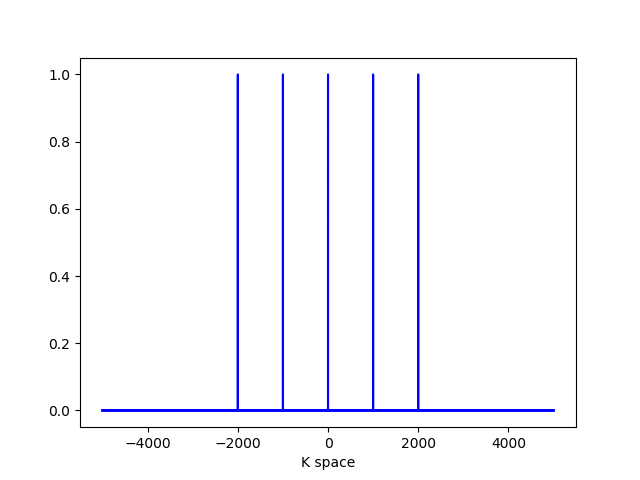
\includegraphics[scale=0.5]{./images/low_rkmax.png}
	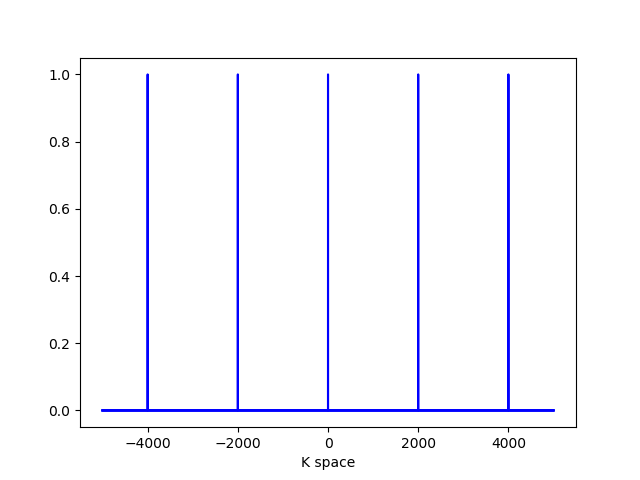
\includegraphics[scale=0.5]{./images/high_rkmax.png}	\caption*{Two case, both with 5 kpoints and different RKMax's.  The plot on the left depicts a smaller RKMax relative to the one on the right.}
\end{figure}


Increasing RKMax allows for higher frequency (more precise) plane waves to be used in the basis set.  These high frequency terms are however more computationally costly (CPU requirements scale as RKMax$^3$) and less essential for describing large features. This is why the RKMax includes the Muffin Tin radius: large atoms only require lower frequency plane waves.  Each atom has an effective RKMax which  is relative to the ratio of its radius and that of the smallest atom.  Choosing very different muffin tin radii for different elements leads to issues as it becomes more difficult to align the surface features of each atom.  \\

Increasing RKMax arbitrarily does not solve the problem either, as: 1. ``approximate numerical linear dependency" occurs at large RKMax values and 2. Calculations become prohibitively expensive.  RKMax should at most be  between 9-10.  

\subsection{Ghostbands}
Ghostbands are an inevitable consequence of investigating lithium with Wien2k.  They manifest as an LAPW2 qtl error during the scf cycles, typically during the first cycle, but sometimes later as well. They are recorded the lapw2(\_n).error files as:  

\begin{lstlisting}
'l2main' - QTL-B.GT.15., Ghostbands, check scf files
\end{lstlisting}

Ghostbands are arise in a number of situations, each of which requires a different solution. Some of these are described below: 

\begin{itemize}	
	
\item \textbf{Muffin Tins badly chosen:} These appear when the muffin tins are too different, or if you ignore everything that \textbf{setrmt} does.  \textbf{Solution:} Diagnose this by running the calculation with the \textbf{setrmt} values (might need to remove the core hole) or make the muffin tins more reasonable (might need to allow core leakage).

\item  \textbf{Local Orbitals need better initial guess:}  Sometimes the starting points for local orbitals are not close enough to the converged values resulting in divergence.  \textbf{Solutions:} Figure out which orbitals are causing the issue by looking in case.scf2(\_n).  The last lines of these files should have a line like this:  

\begin{lstlisting}
:WARN : QTL-B value eq.  99.95 in Band of energy  -0.12674  ATOM=    2  L=  0
\end{lstlisting}

This message also tells us to look in case.in1(\_st) and that the problem is with atom 2 and the L=0 orbital.  In case.in1(\_st),  every independent atom is listed, eg:

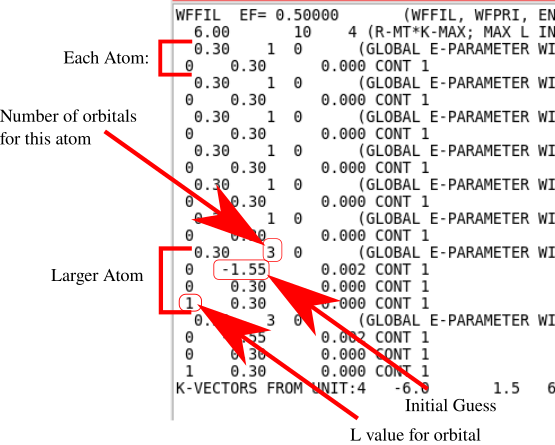
\includegraphics[scale=0.8]{./images/ghostbands.png}




To handle ghostbands, either delete the relevant local orbital line (lines that match the atom and orbital number with energy guesses that are not 0.30) and reduce the number of orbitals for that atom correspondingly.  A more refined option is to adjust the initial guesses to another value, and rerunning \textbf{run\_lapw}.

\end{itemize}


\subsection{NN in Optimization}
Crashes the first scf cycle almost immediately, due to overlapping muffin tins resulting from a decreased cell size.  Solution: decrease all muffin tin sizes before running ``x optimize".


\subsection{GMax Value less than Gmin}

Occurs in \textbf{dstart}, fix is to bump up the Gmax value in case.in2 from 12.00 to 14.00 or 16.00.
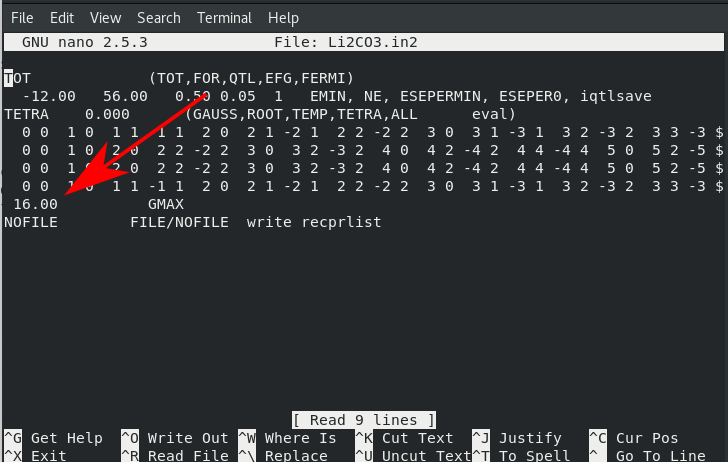
\includegraphics[scale=0.5]{./images/gmax_err.png}

\subsection{Ordering}
If a calculation run apparently unchanged, a possible reason is that all the edits were overwritten by \textbf{init\_lapw}.  The order of a calculation should be: 
\begin{itemize}
	\item Make edits to case.struct file, ie. Muffin Tin Radius
	\item run \textbf{init\_lapw}
	\item  Edit .in files. eg. setting RKMax, dealing with ghostbands, inserting core hole, increasing k points...
	\item \textbf{run\_lapw}
	\item Increase Kpoints, run case specific calculations,  and/or loop back to and run forwards from there (ie increasing k points/RKMax does not require rerunning \textbf{init\_lapw}, but changing muffin tin radii does).
\end{itemize}



\begin{itemize}
	\item \textbf{setrmt}
	\item \textbf{nn}
	\item \textbf{sgroup}
	\item  \textbf{symmery}
	\item \textbf{lstart}
	
\end{itemize}


\end{document}